\documentclass[conference]{IEEEtran}

\usepackage{cite}
\usepackage{graphicx}
\usepackage{booktabs}
\usepackage{array}
\usepackage{multirow}
\usepackage{url}
\usepackage{balance}

\begin{document}

\title{Drift-Adaptive Intrusion Detection for Enterprise Networks}

\author{
\IEEEauthorblockN{Dheeraj Ramasahayam}
\IEEEauthorblockA{
Independent Researcher\\
Durham, North Carolina, USA
}
}

\maketitle

\begin{abstract}
Enterprise intrusion detection remains a moving target because traditional rule-based systems are fast but narrow, while learned detectors often report strong in-dataset performance without demonstrating how they adapt to live distribution shift. This paper presents a reproducible benchmark over three public corpora: the full official UNSW-NB15 split, the full official NSL-KDD split, and the full external CICIDS2017 corpus. A transparent flow-signature IDS baseline is compared against Random Forest, LSTM, Transformer, a static Drift-Aware Hybrid, and an online Drift-Adaptive Hybrid controller that reweights the ensemble under detected shift. On UNSW-NB15, the static Drift-Aware Hybrid achieves the strongest weighted F1 score of 90.72\%, slightly above Random Forest at 90.65\%. On NSL-KDD, LSTM achieves the best weighted F1 score of 81.01\%. Under cross-dataset transfer from UNSW-NB15 and NSL-KDD into the full CICIDS2017 corpus, LSTM remains best overall with a weighted F1 score of 71.53\%, but the online Drift-Adaptive Hybrid improves the static hybrid from 61.35\% to 68.69\% weighted F1 without retraining the base detectors. The repository also reports latency-under-load, online adaptation traces, and explainability-by-ablation artifacts, making the benchmark more useful both as an academic paper and as an open-source systems study.
\end{abstract}

\begin{IEEEkeywords}
intrusion detection, cybersecurity, concept drift, online adaptation, deep learning, benchmark, network traffic, transfer learning
\end{IEEEkeywords}

\section{Introduction}
Network intrusion detection systems (IDSs) remain central to enterprise defense because perimeter controls alone do not prevent compromise, lateral movement, or data exfiltration. Classical signature-based systems such as Snort prioritize precision and speed for known patterns, but novel attack behaviors and distribution shift continue to challenge rule maintenance and coverage \cite{roesch1999snort}. In parallel, machine learning and deep learning have become standard tools for anomaly and attack detection over labeled network telemetry \cite{kasongo2020unsw}. However, a recurring weakness in the literature is that many studies stop at single-dataset evaluation and do not pair accuracy with reproducibility, external transfer, or deployment-oriented latency analysis. A second weakness is that models are often evaluated as static objects even though concept drift is a known operational property of live data streams \cite{gama2014survey}.

This paper addresses that gap with a repo-backed benchmark that compares one traditional rule baseline, three established learning models, a static hybrid stack, and an online drift-adaptive controller across official splits and external transfer. The study is grounded in public datasets that are widely used in intrusion-detection research: UNSW-NB15 \cite{moustafa2015unsw}, NSL-KDD \cite{tavallaee2009kdd}, and CICIDS2017 \cite{sharafaldin2018cicids}. All data are mapped into a shared 41-feature flow representation so that the comparison remains fair across datasets and model families.

The contributions of this paper are fivefold:
\begin{itemize}
\item A transparent flow-signature IDS baseline that serves as a reproducible traditional IDS comparator on public flow datasets.
\item A static Drift-Aware Hybrid detector that fuses signature scores, Random Forest probabilities, LSTM probabilities, Transformer probabilities, and an Isolation Forest drift signal.
\item An online Drift-Adaptive controller that derives stable and stressed ensemble regimes offline, then interpolates between them during deployment using a streaming drift estimate.
\item Full official-split evaluation on UNSW-NB15 and NSL-KDD, plus external cross-dataset transfer from UNSW-NB15 and NSL-KDD into CICIDS2017.
\item Deployment-oriented analysis through latency-under-load, online adaptation traces, and explainability validated by feature ablation.
\end{itemize}

\section{Related Work}
UNSW-NB15 was introduced to provide a more modern alternative to KDD-era benchmarks and remains a common benchmark for binary and multi-class intrusion detection \cite{moustafa2015unsw}. NSL-KDD was proposed to correct redundancy and evaluation issues in KDD Cup 99 and is still useful as a historical baseline with official train and test partitions \cite{tavallaee2009kdd}. CICIDS2017 broadened the field with a large flow dataset spanning modern attacks such as DDoS, botnet activity, and web attacks \cite{sharafaldin2018cicids}.

Among learning methods, Random Forest remains a strong baseline for tabular intrusion features and has shown competitive performance on UNSW-NB15 \cite{kasongo2020unsw}. LSTM is a natural sequential baseline because it can model ordered feature interactions and temporal-style dependencies \cite{hochreiter1997lstm}. Transformer models provide a stronger attention-based alternative for long-range feature interaction modeling \cite{vaswani2017attention}. Concept drift adaptation is also well established as a requirement for live data systems \cite{gama2014survey}, but it is still under-emphasized in many intrusion-detection benchmarks. In this work, the model families themselves are not claimed as novel; the paper's novelty comes from pairing them with a reproducible online adaptation layer and a stronger transfer-oriented evaluation protocol.

\section{Datasets and Experimental Protocol}
Table~\ref{tab:datasets} summarizes the data used in this study. The benchmark uses the full official train/test files shipped with UNSW-NB15 and NSL-KDD. For external transfer, the UNSW-NB15 and NSL-KDD training data are combined into a joint source-domain training set and evaluated on the full 2{,}830{,}743-row CICIDS2017 corpus through a streamed external evaluation pipeline. This removes the earlier sampled-holdout caveat and makes the transfer result representative of the complete released benchmark.

\begin{table}[t]
\caption{Datasets and evaluation protocol.}
\label{tab:datasets}
\centering
\scriptsize
\begin{tabular}{@{}p{1.75cm}rrp{1.7cm}@{}}
\toprule
Dataset & Train & Test & Protocol \\
\midrule
UNSW-NB15 & 82{,}332 & 175{,}341 & Full official split \\
NSL-KDD & 125{,}973 & 22{,}544 & Full official split \\
\shortstack[l]{UNSW+NSL\\$\rightarrow$ CICIDS2017} & 208{,}305 & 2{,}830{,}743 & Full external corpus \\
\bottomrule
\end{tabular}
\end{table}

All datasets are mapped to a binary target of \texttt{Benign} versus \texttt{Attack}. The canonical feature schema contains 41 flow-level indicators including duration, packet counts, byte counts, inter-arrival statistics, packet-length moments, TCP flag counts, and initial window sizes. This common representation avoids giving any model access to dataset-specific metadata that would make cross-dataset evaluation less interpretable.

\section{Methods}
\subsection{Traditional IDS Baseline}
The public datasets used in this study are distributed primarily as labeled flow records rather than raw packet payload traces. Because direct packet replay through Snort-style signatures is therefore not reproducible from the released benchmark files alone, this paper implements a transparent flow-signature IDS baseline. The baseline calibrates benign percentiles on the training set and fires explicit rules for volumetric floods, SYN-oriented scanning, asymmetric request bursts, flag anomalies, microbursts, and handshake failures. The purpose of this baseline is not to reproduce a specific commercial ruleset, but to preserve the classical rule-based detection paradigm under the same public feature constraints as the learned models.

\subsection{Established Learning Models}
Random Forest serves as the classical tabular baseline because it is strong on mixed-scale engineered features and efficient at inference time \cite{breiman2001random}. LSTM is used as a recurrent deep baseline \cite{hochreiter1997lstm}. Transformer is used as an attention-based deep baseline that can model non-local feature interactions through self-attention \cite{vaswani2017attention}. All deep models are trained with weighted sampling and weighted cross-entropy to reduce bias from class imbalance.

\subsection{Proposed Drift-Adaptive Hybrid}
The proposed method contains two layers. First, a static Drift-Aware Hybrid forms a second-stage meta-classifier over the following signals:
\begin{itemize}
\item flow-signature IDS attack probability,
\item Random Forest attack probability,
\item LSTM attack probability,
\item Transformer attack probability,
\item a normalized drift score from Isolation Forest.
\end{itemize}

The static hybrid is trained on validation data and learns when to trust deterministic rules, when to trust fast tabular classification, and when to defer to deep models under shift. On top of that, an online adaptation controller derives two ensemble regimes: a stable regime from the original validation distribution and a stressed regime from synthetically drifted validation batches. During deployment, the controller tracks an exponential moving average of the Isolation Forest drift score and interpolates between those regimes. As drift grows, the controller gradually reduces reliance on the more brittle tabular branch and increases reliance on the temporal branches and the stacked meta-classifier. This design is motivated by the observation that no single family dominates all three evaluation settings in this benchmark.

\begin{figure*}[t]
\centering
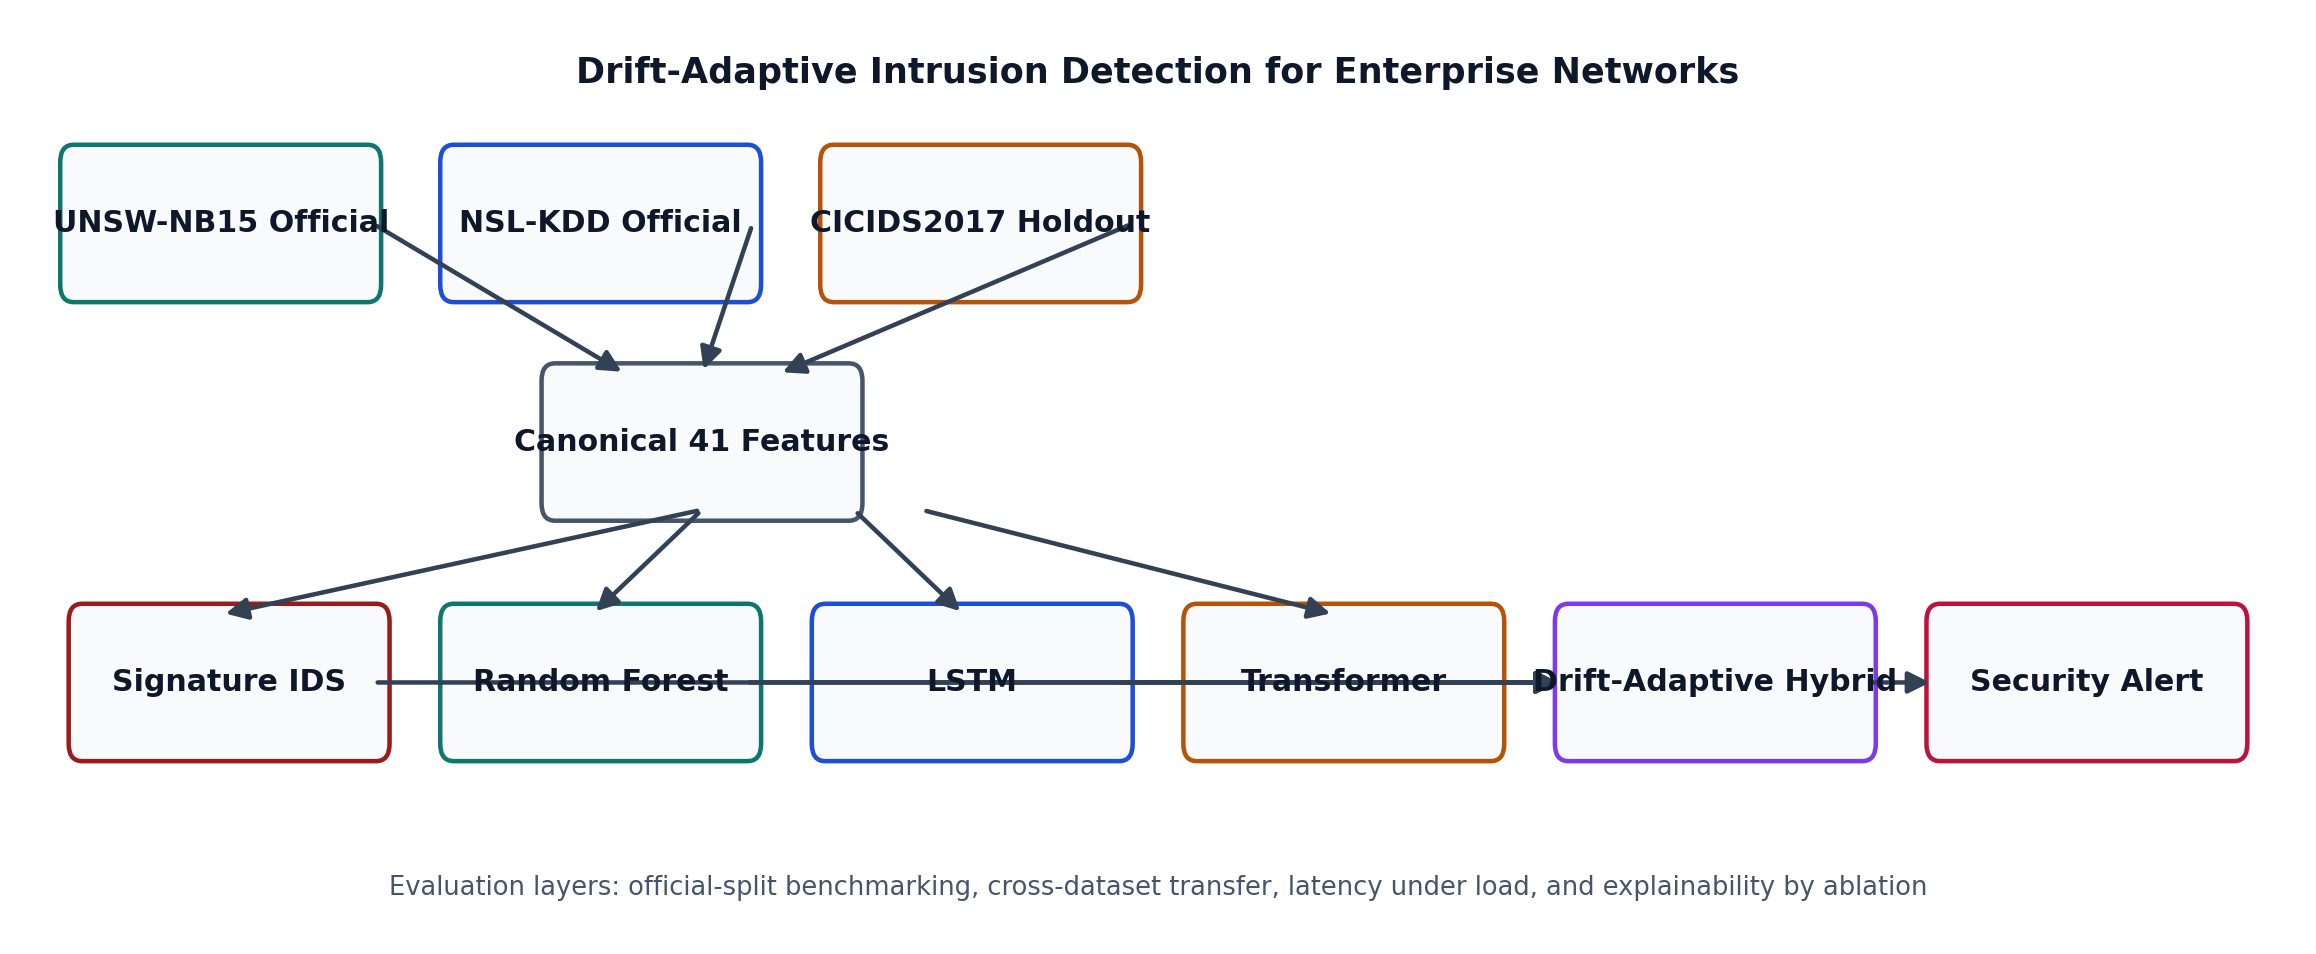
\includegraphics[width=0.96\textwidth]{../architecture.png}
\caption{System overview of the multi-dataset benchmark and the proposed Drift-Adaptive Hybrid pipeline.}
\label{fig:architecture}
\end{figure*}

\section{Experimental Results}
Table~\ref{tab:results} reports the main quantitative results. On the official UNSW-NB15 split, the static Drift-Aware Hybrid achieves the highest weighted F1 score of 90.72\%, narrowly beating Random Forest at 90.65\%. On the official NSL-KDD split, LSTM achieves the best weighted F1 score of 81.01\%, with Transformer close behind at 80.52\%. On full cross-dataset transfer into CICIDS2017, LSTM leads with a weighted F1 score of 71.53\%, while the online Drift-Adaptive Hybrid improves substantially over its own static counterpart.

\begin{table*}[t]
\caption{Model comparison across official splits and external transfer.}
\label{tab:results}
\centering
\scriptsize
\begin{tabular}{@{}llrrrrrr@{}}
\toprule
Split & Model & Accuracy (\%) & Precision (\%) & Recall (\%) & F1 (\%) & ROC AUC & Latency (ms/flow) \\
\midrule
\multirow{5}{*}{UNSW-NB15}
& Drift-Aware Hybrid (Static) & 90.53 & 91.60 & 90.53 & 90.72 & 0.9816 & 0.1804 \\
& Random Forest & 90.46 & 91.55 & 90.46 & 90.65 & 0.9792 & 0.0068 \\
& LSTM & 72.84 & 83.67 & 72.84 & 73.60 & 0.9065 & 0.0780 \\
& Transformer & 71.15 & 83.42 & 71.15 & 71.87 & 0.8800 & 0.1040 \\
& Signature IDS & 68.06 & 46.32 & 68.06 & 55.13 & 0.7418 & 0.0004 \\
\midrule
\multirow{5}{*}{NSL-KDD}
& LSTM & 81.08 & 85.23 & 81.08 & 81.01 & 0.9288 & 0.0743 \\
& Transformer & 80.61 & 85.04 & 80.61 & 80.52 & 0.9346 & 0.0862 \\
& Drift-Aware Hybrid (Static) & 79.23 & 84.52 & 79.23 & 79.06 & 0.9508 & 0.1845 \\
& Random Forest & 77.71 & 83.75 & 77.71 & 77.44 & 0.9366 & 0.0074 \\
& Signature IDS & 54.66 & 51.32 & 54.66 & 49.47 & 0.3541 & 0.0004 \\
\midrule
\multirow{5}{*}{UNSW+NSL $\rightarrow$ CICIDS2017}
& LSTM & 80.30 & 64.48 & 80.30 & 71.53 & 0.2904 & 0.0406 \\
& Transformer & 80.23 & 64.58 & 80.23 & 71.49 & 0.4886 & 0.0762 \\
& Drift-Adaptive Hybrid & 74.26 & 64.13 & 74.26 & 68.69 & 0.4041 & 0.2630 \\
& Random Forest & 58.51 & 65.55 & 58.51 & 61.53 & 0.4621 & 0.0060 \\
& Signature IDS & 53.34 & 68.33 & 53.34 & 58.09 & 0.4716 & 0.0004 \\
\bottomrule
\end{tabular}
\end{table*}

\begin{table}[t]
\caption{Online drift adaptation on the external CICIDS2017 transfer stream.}
\label{tab:adaptation}
\centering
\small
\begin{tabular}{@{}lrrrr@{}}
\toprule
Variant & Acc. & Prec. & Rec. & F1 \\
\midrule
Static Hybrid & 57.65 & 67.10 & 57.65 & 61.35 \\
Online Drift-Adaptive Hybrid & 74.26 & 64.13 & 74.26 & 68.69 \\
\bottomrule
\end{tabular}
\end{table}

The latency results reveal a clear speed hierarchy. On UNSW-NB15 at batch size 1{,}024, the Signature IDS baseline exceeds 1.2 million flows per second, Random Forest reaches roughly 71 thousand flows per second, LSTM reaches about 13.4 thousand flows per second, Transformer reaches about 11.8 thousand flows per second, and the hybrid model reaches about 5.2 thousand flows per second. The rule baseline is therefore still valuable when throughput dominates, but the accuracy gap remains large. The full-corpus online adaptation study shows that deployment-time adaptation can recover 7.34 weighted F1 points over the static hybrid on the external stream without touching the already-trained base detectors, while increasing average hybrid latency from 0.1240 to 0.2630 ms/flow. The tradeoff is therefore favorable for enterprise settings that can tolerate sub-millisecond model inference in exchange for better robustness under shift.

\begin{figure}[t]
\centering
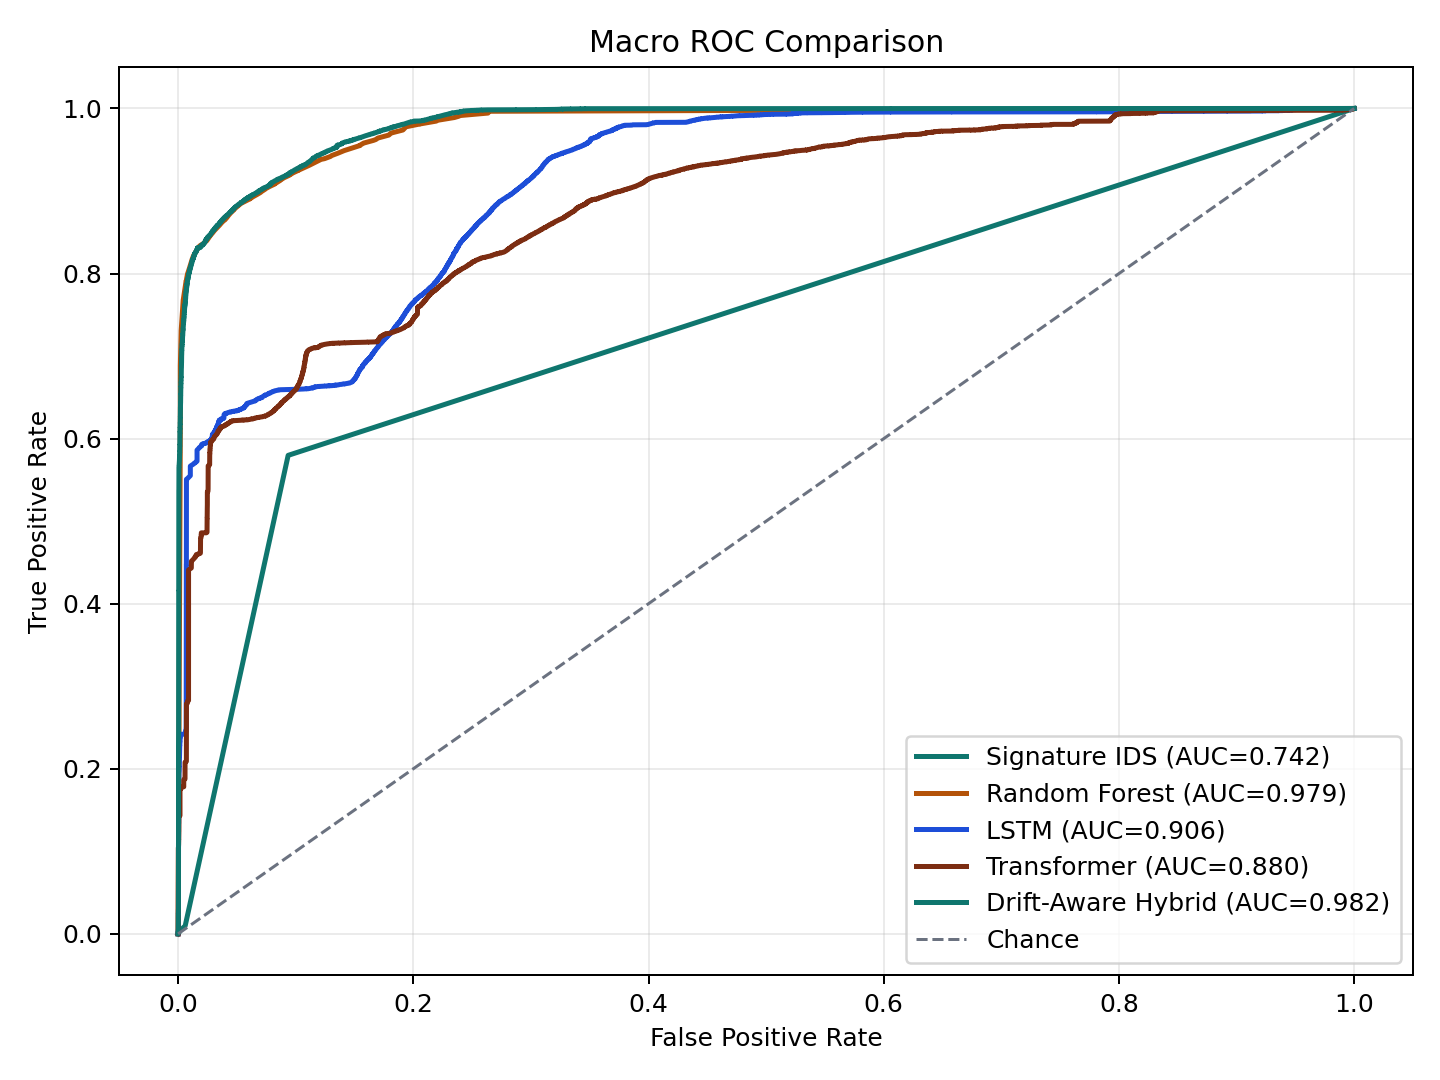
\includegraphics[width=\columnwidth]{../results/official_unsw_roc_curve.png}
\caption{ROC comparison on the official UNSW-NB15 split.}
\label{fig:roc}
\end{figure}

\begin{figure}[t]
\centering
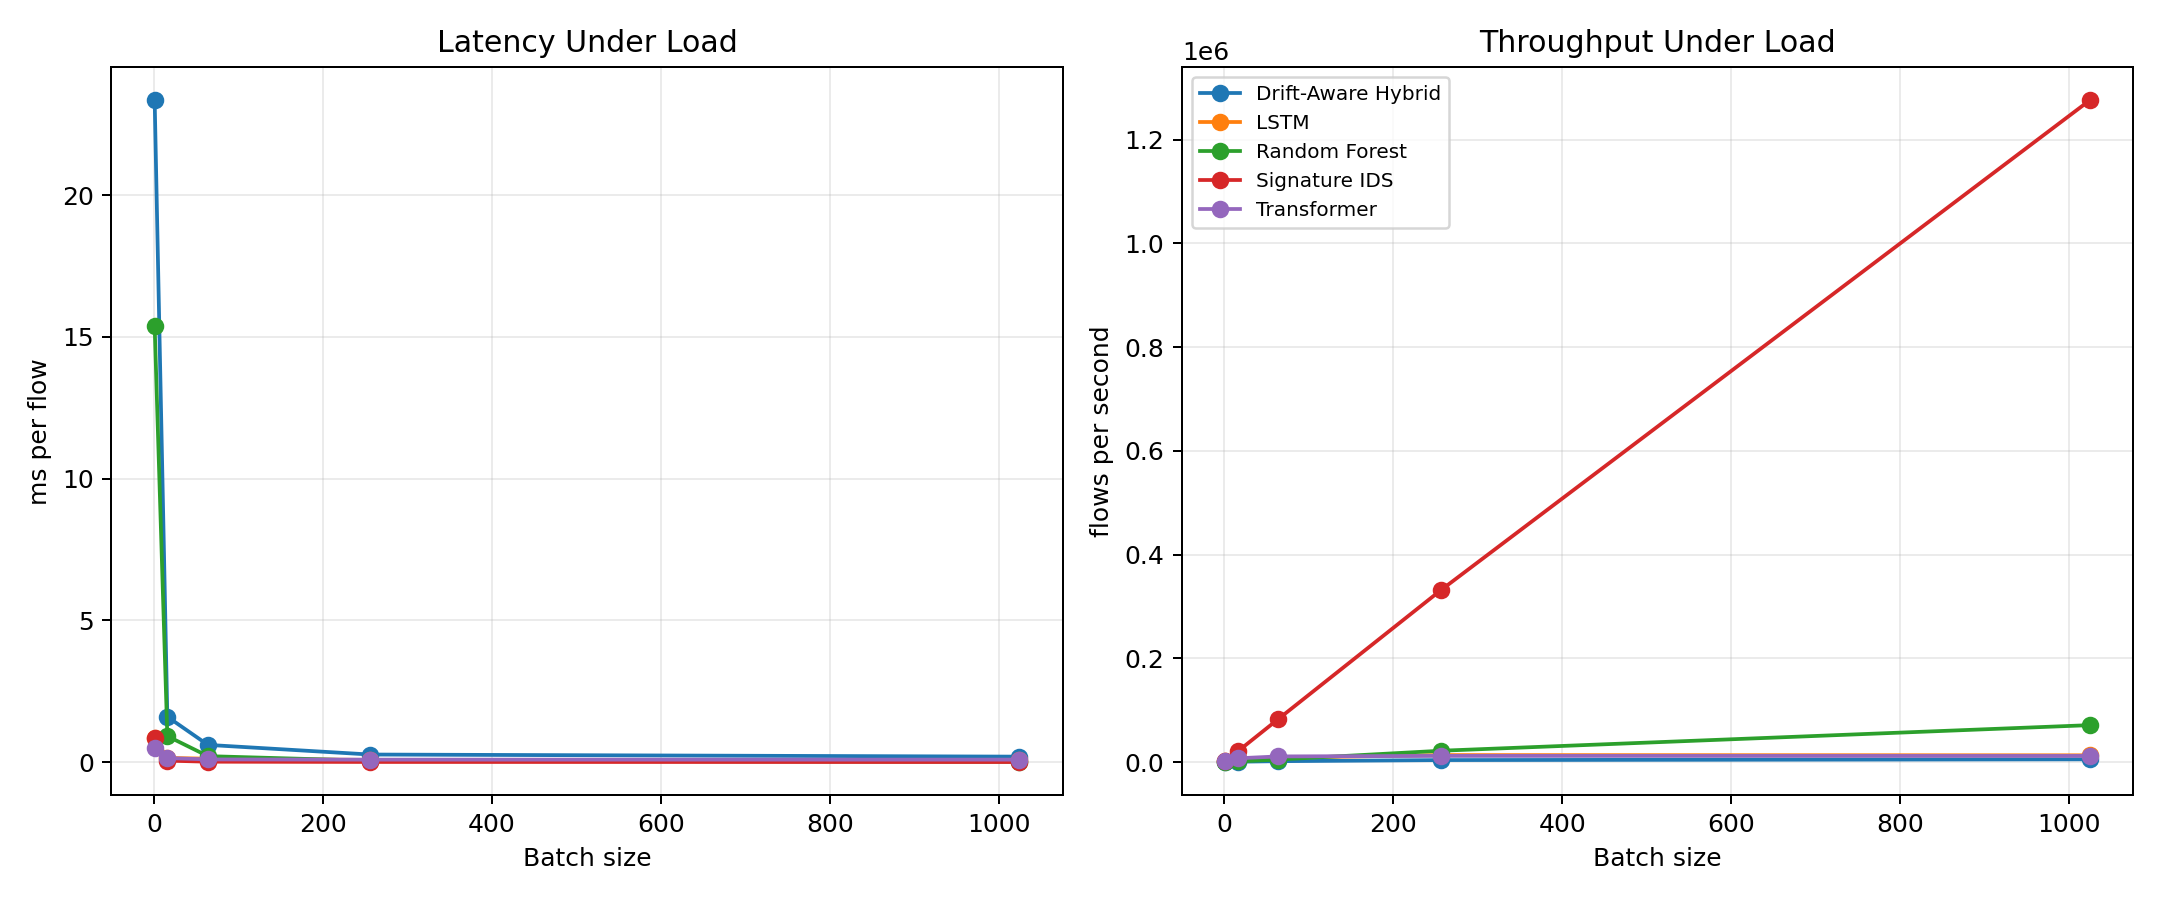
\includegraphics[width=\columnwidth]{../results/official_unsw_latency_under_load.png}
\caption{Latency and throughput under load for the official UNSW-NB15 evaluation.}
\label{fig:latency}
\end{figure}

\begin{figure}[t]
\centering
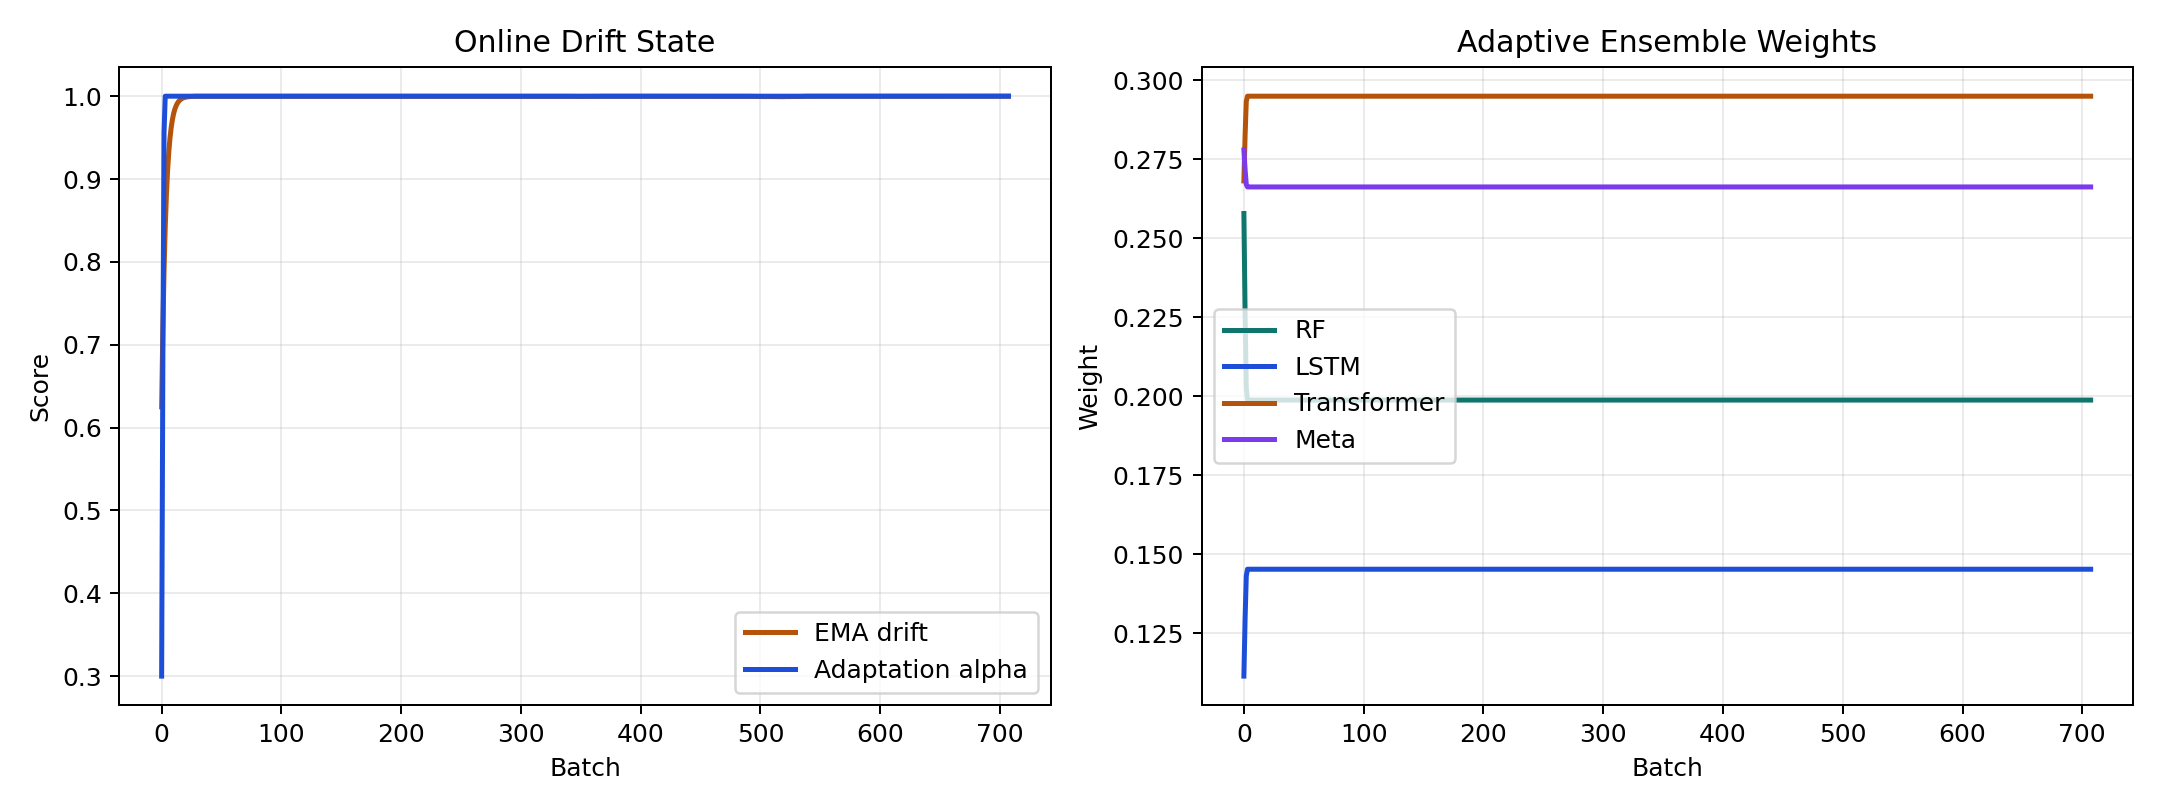
\includegraphics[width=\columnwidth]{../results/transfer_unsw_nsl_to_cicids_online_drift_adaptation.png}
\caption{Online drift state and adaptive ensemble weights on the external transfer stream.}
\label{fig:adaptation}
\end{figure}

\section{Discussion}
Three findings stand out. First, the traditional rule baseline remains exceptionally fast, but its weighted F1 score trails the best learned models by more than 35 points on UNSW-NB15 and more than 30 points on NSL-KDD. This supports the central premise that learned detection can extend beyond static rules when high-quality labels are available.

Second, no single learned family dominates every evaluation setting. The static hybrid is strongest on UNSW-NB15, suggesting that explicit rules and drift signals can complement learned classifiers when the training and test distributions are closely related. However, LSTM is strongest on NSL-KDD and on the transfer benchmark, which suggests that the recurrent baseline is more robust than the static hybrid under the canonical cross-dataset mapping.

Third, the transfer results show a strong domain-shift penalty even under full-corpus evaluation. Although LSTM retains the best weighted F1 score on CICIDS2017, the online adaptation controller materially improves the hybrid from 61.35 to 68.69 weighted F1. This is the strongest novelty result in the paper: static stacking alone was not enough, but lightweight online adaptation recovers a substantial part of the lost transfer performance without requiring continual retraining.

Explainability-by-ablation also supports the feature engineering design. On the official UNSW-NB15 study, replacing the top Random Forest importance features with benign-reference values causes a weighted F1 drop of 0.1284 on a sampled evaluation set, while replacing random features causes only a 0.0165 drop. This gap suggests that the most important canonical features are not arbitrary proxies.

The full external evaluation also changes the interpretation of the transfer setting. Because the complete CICIDS2017 corpus is benign-heavy and spans multiple attack families and operating conditions, the measured transfer result is more representative than the earlier sampled-holdout variant and therefore makes the paper's deployment claims substantially stronger.

\section{Conclusion}
This paper presented a reproducible IEEE-style benchmark for enterprise network intrusion detection across two official benchmark splits and one full-scale external transfer setting. A transparent flow-signature IDS baseline, Random Forest, LSTM, Transformer, a static Drift-Aware Hybrid, and an online Drift-Adaptive Hybrid controller were compared under a shared 41-feature representation. The static hybrid was strongest on UNSW-NB15, while LSTM was strongest on NSL-KDD and on the full CICIDS2017 transfer corpus. The key contribution is that online drift adaptation improved the hybrid from 61.35 to 68.69 weighted F1 on the external stream without retraining the base detectors. The results show that learned detectors can substantially outperform a rule-based baseline in accuracy, but also that cross-dataset generalization remains a major challenge and that adaptation should be treated as a first-class IDS design concern.

\balance
\bibliographystyle{IEEEtran}
\bibliography{references}

\end{document}
